\documentclass{beamer}

\usepackage[latin1]{inputenc}
\usepackage[T1]{fontenc}
\usepackage[frenchb]{babel}
\usepackage{lmodern}
\usepackage{graphicx}

\usetheme{Ilmenau}
\usecolortheme{seagull}

\logo{
\includegraphics[height=10mm]{ur1.png}}

\title{Soutenance de TIPE}
\subtitle{Comment la reconnaissance faciale du conducteur peut-elle am\'eliorer sa s�curit\'e au volant ?}
\author{S\'ebastien Blin, Pierre-Henri Collin, Amaury Louarn}
\institute{Universit\'e de Rennes 1}
\date{8 Avril 2014}

\AtBeginSection[]
{
  \begin{frame}
  \frametitle{Sommaire}
  \tableofcontents[currentsection, currentsubsections]
  \end{frame} 
}

\begin{document}
	\begin{frame}
		\titlepage
	\end{frame}
	
	\section{Introduction}
	\begin{frame}
		\frametitle{Introduction}
	\end{frame}
	\section{Reconnaissance faciale}
	\begin{frame}
		\frametitle{Impl\'ementation choisie}
	\end{frame}
	\begin{frame}
		\frametitle{Pourquoi ce choix d'impl\'ementation}
	\end{frame}
	
	\section{Reconnaissance des \'emotions}
	\subsection{Expressions faciales}
	\begin{frame}
		\frametitle{Les 6 \'emotions primaires}
		\begin{figure}
			\begin{center}
				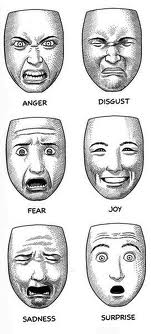
\includegraphics[scale=0.5]{images/primaryexp}
			\end{center}
		\end{figure}
	\end{frame}
	\begin{frame}
		\frametitle{\'Emotions \`a d\'etecter}
	\end{frame}
	\subsection{Impl\'ementation}
	\begin{frame}
		\frametitle{Reconnaissance de la bouche}
	\end{frame}
	\begin{frame}
		\frametitle{Reconnaissance des yeux}
	\end{frame}
	\subsection{Pourquoi ce choix~?}
	\begin{frame}
		\frametitle{Pourquoi ce choix d'impl\'ementation}
	\end{frame}
	
	\section{D\'emonstration}
	\begin{frame}
		\frametitle{}
	\end{frame}
	
	\section{Conclusion}
	\begin{frame}
		\frametitle{Conclusion}
	\end{frame}
	\begin{frame}
		%\frametitle{Questions}
		\begin{block}{}
			\begin{center}
				Des questions?
			\end{center}
		\end{block}
	\end{frame}
\end{document}
	